\chapter{Introduction}\label{chap:introduction}
Semantic segmentation is a popular and promising research topic in the field of computer vision, and particularly for autonomous vehicles.
By semantically segmenting the scene, the autonomous vehicle is able to identify various objects in field of view, which is important for autonomous vehicle and robots to safely navigate an environment.
Generally, most implementations attempt to segment road surfaces but in this thesis, we propose the segmentation of curbs and curb cuts to allow safer sidewalk navigation.

The Europa project has resulted in the Obelix robotic platform, which has already been demoed to successfully perform pedestrian navigation in urban environments~\cite{europa}\cite{obelix-slam}.
We propose to add to this platform the ability to detect curbs and curb cuts using semantic segmentation.
The Obelix platform is the result of a joint project to build a robotic platform capable of robotic navigation~\cite{europa}. 
In its current state, Obelix is already capable of localization and navigation using a map generated using LIDAR, but it is unable to determine what surface type it is driving on, e.g. asphalt, concrete, carpet, etc.~\cite{jannik}.
Research is currently underway to extend its pathfinding ability, using the onboard cameras to classify terrains that Obelix will encounter~\cite{jannik}.
This work specifically aims to add to said research by additionally identifying curbs and curb cuts, providing constraints for the route planner.
This will allow the route planner to identify curbs, which it cannot traverse, and curb cuts, which it can.

\begin{figure}
	\centering
	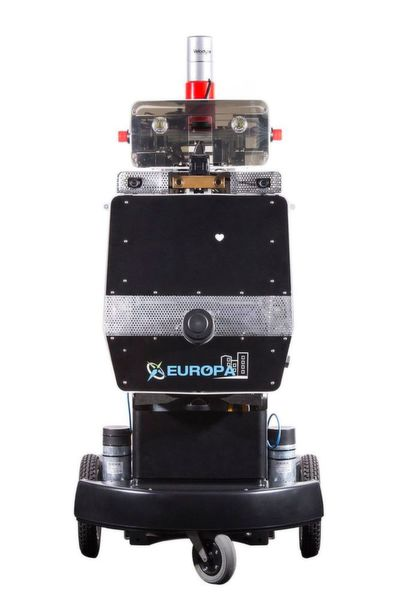
\includegraphics[width=.3\textwidth]{figures/introduction/obelix.jpg}
	\caption{The Obelix Robot platform developed by the Europa project. We plan to extend its path finding capabilities using the work in this thesis.}
\end{figure}

The aim of this work is thus to implement a deep learning model capable of the semantic segmentation of curbs and curb cuts using a single camera image.
To this end, we propose the implemention of a convolutional neural network (CNN) based on the paper "Encoder-Decoder with Atrous Separable Convolution for Semantic Image Segmentation" by Chen Liang Chieh et al~\cite{deeplab}.
We additionally use a modified loss function based on cross entropy loss.
We call our proposed implementation CurbNet.

This thesis begins by discussing related works in chapter \ref{chap:relatedwork}. 
Background knowledge that will be important in understanding the approach taken and the work in general will be discussed in chapter \ref{chap:background}.
The approach is then discussed in detail in chapter \ref{chap:approach}, with a discussion regarding the architecture the model uses and the loss function used.
The experiments performed are discussed in chapter \ref{chap:experiments} and their results analyzed in section \ref{section:experiments-results}.
Finally, a conclusion and a short discussion of potential future research is presented in chapter \ref{chap:conclusion}.